\chapter{Gestione dei processi}

Il compito fondamentale di un sistema operativo è la gestione dei processi, ovvero eseguire diverse computazioni. Infatti un sistema operativo deve poter permettere l'esecuzione alternata di processi multipli; assegnare le risorse ai processi; permettere ai processi di scambiarsi informazioni; permettere la sincronizzazione tra processi.

\begin{redbar}
    Un \textbf{processo} è a tutti gli effetti un'istanza di un programma in esecuzione caratterizzata da una sequenza di istruzioni, da uno stato corrente e da un insieme associato di risorse.
\end{redbar}

Va specificato che per esecuzione di un processo si intende l'esecuzione di un programma che ancora non è terminato. Questo non significa che il processo sia effettivamente in esecuzione su un processore, infatti la decisione di esecuzione di un processo è uno dei compiti fondamentali di un sistema operativo. 

Solo eseguendo un programma si crea un processo. Nei sistemi operativi moderni il programma è sempre registrato su un disco rigido, fanno eccezioni i processi creati dal sistema operativo stesso.

\section{Stati di un processo}
Ogni processo ha tre macro-fasi: \textit{creazione}, \textit{esecuzione}, \textit{terminazione}. La terminazione, se presente, può essere o esplicitamente prevista (es. click sulla X della finestra), oppure non prevista (in caso di errori).

\begin{wrapfigure}{r}{0.20\linewidth}
\vspace{-20pt}
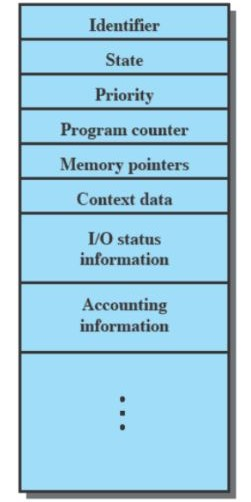
\includegraphics[width=1\linewidth]{images/process_control_block.JPG}
    \label{fig:process_control_block}
\vspace{-30pt}
\end{wrapfigure}
Finché un processo è in esecuzione ha associato un \textit{Process Control Block} creato dal sistema operativo. 
Questo block contiene sufficienti informazioni per permettere al sistema operativo di gestire più processi contemporaneamente. Queste informazioni sono: un \textit{identificatore} per differenziare i processi; uno \textit{stato} (es. running...); \textit{priorità}; \textit{hardware context} contiene il valore corrente dei registri della CPU; dei \textit{puntatori alla memoria} che definiscono l'immagine del processo; delle \textit{informazioni sullo stato dell'I/O}; delle eventuali \textit{informazioni di accounting}.

Il comportamento di un processo è caratterizzato dalla sequenza di istruzioni che vengono eseguite, questa sequenza è detta \textit{trace} (traccia). Il \textit{dispatcher}, invece, è un piccolo programma contenuto in memoria che ha il compito di sospendere un processo per eseguirne un altro.\\\\

\begin{Example}{Gestione dei processi}{}
    \textit{Si considerino 3 processi in esecuzione tutti in memoria compreso il dispatcher.}
    
    \begin{minipage}{\textwidth}
        \centering
        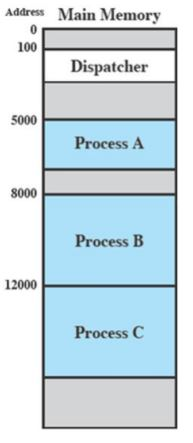
\includegraphics[height=7cm]{images/esempio_traccia1.JPG}
        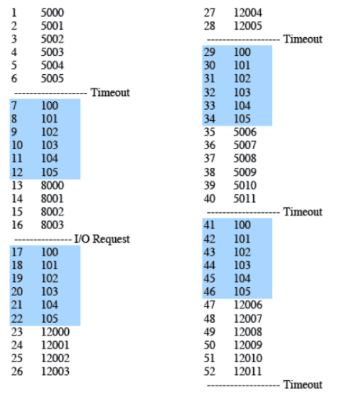
\includegraphics[height=7cm]{images/esempio_traccia2.JPG}
        \captionof{figure}{Esempio di esecuzione di un programma}
        \label{fig:esempio-traccia}
    \end{minipage}
    La sequenza di istruzioni sul processore non è sequenziale come mostrato nella figura di sinistra, ma dobbiamo immaginare una coda di processi in attesa e un dispatcher che muove i processi dalla CPU alla coda e viceversa, finché un processo non viene completato.
\end{Example}

In ogni sistema operativo ci sono $n\geq1$ processi, infatti come minimo c'è un processo master (interfaccia grafica o testuale) che attende comandi dall'utente e non può essere terminato a meno che non viene spento il computer. Nel momento in cui l'utente esegue un comando quasi sempre si crea un nuovo processo. Questo concetto, secondo cui un processo ne crea un altro, viene chiamato \textit{process spawning}. Il processo padre è il processo originale che crea il processo figlio passando da $n$ a $n+1$ processi in esecuzione.

La terminazione di un processo può avvenire per normale completamento, (\textit{HALT}) generando un'interruzione che viene gestita dall'handler del sistema operativo, o per uccisioni (\textit{kill}) dal sistema operativo stesso, per errori, o dall'utente, tramite GUI.

A questo punto i cinque stati dei processi sono divisi in: creazione, terminazione ed esecuzione che comprende \textit{Running}, \textit{Ready} o \textit{Blocked} quando il processo viene messo in attesa (ad es. per aspettare una riposta dai dispositivi di I/O).
\begin{figure}[h]
    \centering
    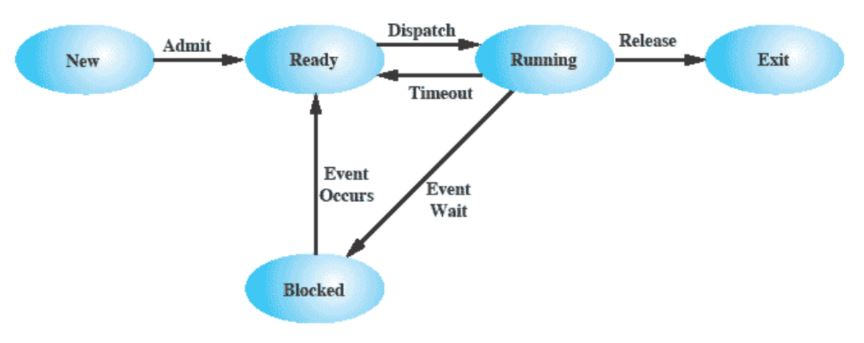
\includegraphics[height=3.5cm]{images/stati-dei-processi1.JPG}
    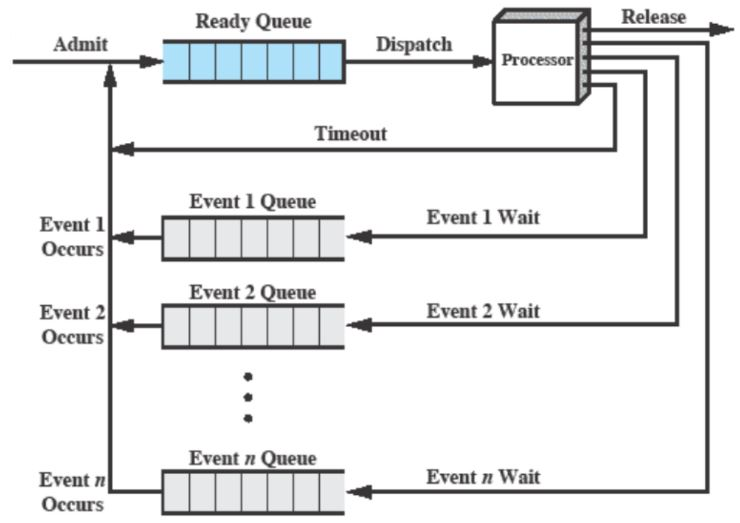
\includegraphics[height=3.5cm]{images/stati-dei-processi2.JPG}
    \caption{Stati di un processo}
    \label{fig:stati-dei-processi}
\end{figure}

A livello di strutture dati troviamo $n$ code: una per i processi Ready che possono andare direttamente in esecuzione nel processore e $n-1$ code per i processi Blocked che fungono da code di attesa. I sistemi operativi, infatti, non hanno una coda per tutti i casi di block ma ne hanno una per ogni evento bloccante in modo da aumentare l'efficienza del sistema.

Molti processi che finiscono in attesa stanno di fatto occupando spazio prezioso in RAM, per questo motivo vengono spostati su disco così da liberare la memoria, questi processi vengono chiamati processi sospesi (\textit{Suspended}). Ai cinque stati originali se ne aggiungono due: (\textit{Blocked/Suspend}) e (\textit{Ready/Suspend}).
\begin{figure}[h]
    \centering
    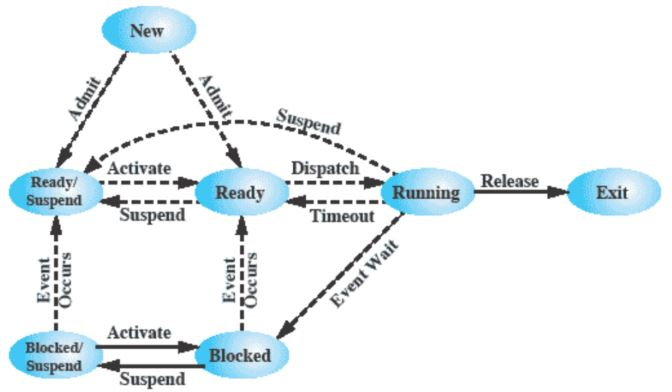
\includegraphics[width=0.7\linewidth]{images/stati-dei-processi3.JPG}
    \caption{Stati sospesi di un processo}
    \label{fig:stati-dei-processi-sospesi}
\end{figure}

Notiamo ora che quando viene creato un nuovo processo c'è subito una scelta da fare, ovvero inserire il processo in RAM con stato Ready per essere scelto dal dispatcher oppure su disco con stato Ready/Suspend.

Abbiamo visto che i processi vengono sospesi per risparmiare risorse di memoria, in realtà i motivi per sospendere un processo possono essere diversi: \textit{swapping} quando il sistema operativo ha bisogno di rilasciare abbastanza memoria da portarci dentro un processo Ready; il sistema operativo sospetta che il processo stia causando problemi; per richieste utente interattive come il debugging; il processo viene eseguito periodicamente; il padre vorrebbe poter sospendere l'esecuzione del figlio per esaminarlo, modificarlo o coordinare l'attività dei figli.

\section{Descrizione di un processo}
Un altro dei compiti principali di un sistema operativo è la gestione dell'uso delle risorse da parte dei processori. Poiché il sistema operativo deve gestire sia i processi che le risorse, deve conoscere lo stato interno di entrambe le entità, a tal proposito, per ogni entità costruisce o mantiene una o più tabelle.
\begin{figure}[h]
    \centering
    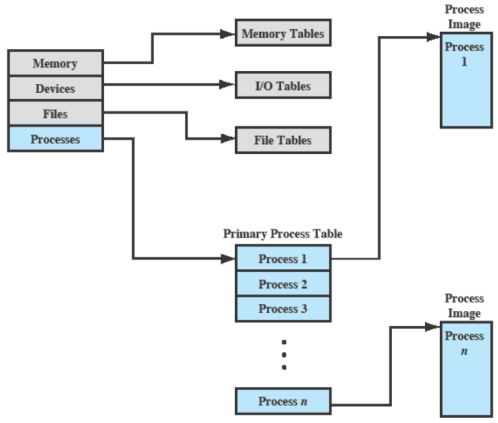
\includegraphics[width=0.5\linewidth]{images/tabelle-di-controllo.JPG}
    \caption{Tabelle di controllo del sistema operativo}
    \label{fig:tabelle-di-controllo}
\end{figure}

In questa sezione ci soffermeremo solamente sulle tabelle dei processi e le altre tabelle saranno approfondite nei capitoli dedicati.

Lo stato interno di una \textit{tabella dei processi} contiene: uno \textit{stato} corrente (Ready, Running, Blocked...); un \textit{identificatore} per distinguere i processi; una \textit{locazione di memoria}; altre informazioni utili. Molte di queste informazioni si trovano nel \textit{Process Control Block} (PCB) e vengono chiamate \textit{attributi} di un processo, mentre il processo vero e proprio chiamato \textit{Process Image} (immagine del processo), per ovvi motivi di spazio, non si trova nel PCB ma in memoria. La Process Image è l'insieme del programma sorgente, dati, stack delle chiamate e PCB. Anche l'esecuzione di una sola istruzione cambia l'immagine del processo perché vengono modificati uno o più registri o celle di memoria.

\subsection*{Attributi di un processo}
Gli attibuti di ciascun blocco di controllo possono essere raggruppate in tre categorie: identificazione; stato; controllo.
\begin{enumerate}
    \item Ad ogni processo è assegnato un numero identificativo \textit{PID} (Process IDentifier). Questo identificativo è così importante che  molte tabelle del sistema operativo, per realizzare i collegamenti con la tabella dei processi, usano direttamente i PID. Fanno parte degli identificatori anche il processo padre (Parent PID, o PPDI) e l'utente che ha eseguito il processo;
    \item Lo stato del processore, da non confondere con lo stato del processo, è formato dal contenuto dei registri del processore stesso;
    \item Fanno parte invece delle informazioni di controllo: 
    \begin{itemize}
        \item \textit{Informazioni per il controllo del processo}: lo stato (Ready, Suspended, Blocked...); la priorità; informazioni sullo scheduling; l'evento da attendere per tornare ad essere Ready;
        \item \textit{Supporto per strutture dati}: puntatori ad altri processi;
        \item \textit{Comunicazioni tra processi}: flag, segnali, messaggi per supportare comunicazioni tra processi;
        \item \textit{Permessi speciali};
        \item \textit{Gestione della memoria}: puntatori ad aree di memoria che gestiscono l'uso della memoria virtuale, ad es. pagine virtuali attualmente in uso;
        \item \textit{Uso delle risorse}: file aperti, uso di risorse (compreso il processore).
    \end{itemize}
\end{enumerate}

\section{Controllo di un processo}
Abbiamo visto come la maggior parte dei processori supporta almeno due modalità di esecuzione: modo di sistema (\textit{kernel}) in cui si ha il pieno controllo del sistema (si può eseguire qualsiasi istruzione o accedere a qualsiasi locazione di memoria); modo utente (\textit{user}) è la modalità di esecuzione dei programmi utente dove molte operazioni sono vietate.

Le operazioni effettuate dal kernel sono: la \textit{gestione dei processi} tramite PCB che permettono la creazione, terminazione, sheduling, dispatching, process switching, sincronizzazione e comunicazione tra processi; la \textit{gestione della memoria principale} che prevede l'allocazione/de-allocazione di spazio per i processi e la gestione della memoria virtuale; la \textit{gestione dell'I/O} per la gestione dei buffer e delle cache e l'assegnazione delle risorse di I/O ai processi; le \textit{funzioni di supporto} per la gestione degli interrupt/eccezioni, accounting e monitoraggio.

In un sistema di questo tipo, dove molti processi hanno necessità di I/O, nasce l'esigenza di passare da modalità kernel a quella utente e viceversa. L'idea è molto semplice: un processo utente inizia sempre in modalità utente; passa a modalità sistema a seguito di un interrupt, in questa fase l'hardware prima di invocare l'interrupt handler cambia la modalità da utente a sistema; l'ultima istruzione dell'interrupt handler, prima di restituire il controllo al processo utente, effettua nuovamente lo switch in modalità utente. Con questo schema, un processo utente può cambiare la modalità a sé stesso, ma solo per eseguire software di sistema.
Per richiedere un servizio a livello kernel del sistema operativo si usano delle chiamate di sistema (o \textit{system call}), in effetti anche la creazione di un nuovo processo è una system call.

Per creare un processo il sistema operativo deve: assegnare al processo un PID unico; allocargli spazio in memoria principale; inizializzare il process control block; inserire il processo nella giusta coda (ready o ready/suspended); creare o espandere altre strutture dati.

Lo switching tra processi, invece, può essere scatenato da varie cause: interruzione esterna all'esecuzione dell'istruzione corrente (include i timer per evitare la prolungata esecuzione di un processo); eccezione associata all'istruzione corrente; chiamata esplicita al sistema operativo (system call). Per eseguire lo switching bisogna seguire vari passaggi in kernel mode: salvare il contesto del programma (registri e PC); aggiornare il process control block, attualmente in running; spostare il process control block nella coda appropriata (ready, blocked, ready/suspend); scegliere un altro processo da eseguire; aggiornare il process control block del processo selezionato; aggiornare le strutture dati per la gestione della memoria; ripristinare il contesto del processo selezionato.

\section{Esecuzione del sistema operativo}
A questo punto nasce spontanea una domanda: \textit{il sistema operativo è un processo?} Abbiamo definito il sistema operativo come un insieme di programmi eseguiti sul processore che permette agli altri programmi di andare in esecuzione, per poi riprendere il controllo tramite interrupt. In questo senso il sistema operativo è a tutti gli effetti un processo, \textit{ma quindi da chi viene controllato?}

\begin{wrapfigure}{r}{0.40\linewidth}
\vspace{0pt}
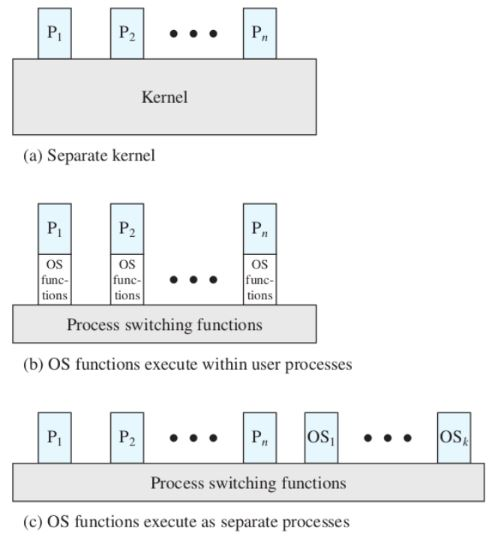
\includegraphics[width=1\linewidth]{images/esecuzione-sistema-operativo.JPG}
    \label{fig:esecuzione-sistema-operativo}
\vspace{-30pt}
\end{wrapfigure}
In realtà dipende dal tipo di sistema operativo: ci sono sistemi operativi, meno recenti, che usano il kernel separato, altri che usano delle funzioni eseguite all'interno del processo utente e altri ancora che uniscono le due modalità.
\begin{itemize}
    \item[a.] Il kernel viene eseguito al di fuori dei processi e il sistema operativo è eseguito come un'entità separata, con privilegi più elevati che ha una sua zona di memoria dedicata per i dati, per il codice sorgente e per lo stack.

\item[b.] Nei sistemi che utilizzano l'esecuzione all'interno dei processi utente, il sistema operativo viene eseguito nel contesto di un processo utente e non c'è bisogno di un process switch ma basta cambiare modalità di esecuzione da utente a sistema.

\item[c.] Nel sistema operativo basato sui processi, invece, tutti gli aspetti sono visti come dei processi (tranne le funzioni di switch). Il sistema operativo stesso è implementato come un insieme di processi di sistema con privilegi più alti.
\end{itemize}

\section{Gestione dei processi UNIX SVR4}
UNIX SVR4 usa il modello dove la maggior parte del sistema operativo viene eseguito all'interno dei processi utente. UNIX utilizza due categorie di processi: processi di sistema eseguiti in modalità kernel e processi utente per eseguire programmi ed utilità.
\begin{figure}[h]
    \centering
    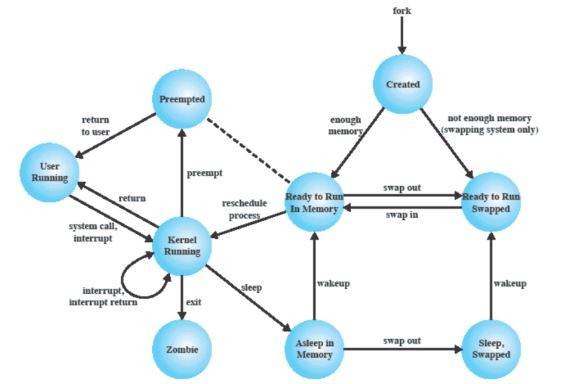
\includegraphics[width=0.70\linewidth]{images/stati-unix.JPG}
    \caption{Stati dei processi in UNIX}
    \label{fig:stati-unix}
\end{figure}
Il diagramma degli stati dei processi (vedi Figura \ref{fig:stati-unix}) è diviso in nove stati diversi che comprendono: \textit{User Running} in esecuzione in modalità utente; \textit{Kernel Running} in esecuzione in modalità kernel o sistema; \textit{Ready to Run in Memory} può andare in esecuzione non appena il kernel lo seleziona; \textit{Asleep in Memory} non può essere eseguito finchè un qualche evento non si manifesta e il processo è in memoria; \textit{Ready to Run Swapped} può andare in esecuzione (non è in attesa di eventi esterni), ma prima dovrà essere portato in memoria; \textit{Sleeping Swapped} non può essere eseguito finché un qualche evento non si manifesta e il processo non è in memoria primaria; \textit{Preempted} il kernel ha appena tolto l'uso del processore a questo processo (preemption), per fare un context switch; \textit{Created} appena creato, ma ancora non pronto all'esecuzione; \textit{Zombie} terminato, ma resta nelle tabelle dei processi perché il processo che l'ha creato possa prendersi il suo valore di ritorno.

Un insieme di strutture dati forniscono al sistema operativo le informazioni per gestire i processi. Queste informazioni sono raggruppate in livello utente, livello registro e livello di sistema.

A livello utente trovamo: \textit{Process text} il codice sorgente (in linguaggio macchina) del processo; \textit{Process data} sezione di dati del processo dove vengono mappati i valori delle variabili; \textit{User stack} ovvero lo stack delle chiamate del processo; \textit{Shared Memory}, la memoria condivisa con altri processi, usata per le comunicazioni tra processi.

Il livello registro contiene: \textit{Program counter}, l'indirizzo della prossima istruzione del process text da eseguire; \textit{Processor status register}, il registro di stato del processore, relativo a quando è stato swappato l'ultima volta; \textit{Stack pointer} è il puntatore alla cima dello user stack; \textit{General purpose registers} rappresenta il contenuto dei registri accessibili al programmatore, relativo a quando è stato swappato l'ultima volta.

Il livello sistema ha:\textit{ Process table entry}, il puntatore alla tabella di tutti i processi, dove individua quello corrente; \textit{U area} contiene le informazioni per il controllo del processo; \textit{Per process region table} definisce il mapping tra indirizzi virtuali ed indirizzi fisici (page table); \textit{Kernel stack} è lo stack delle chiamate, separato da quello utente, usato per le funzioni da eseguire in modalità sistema.
\begin{figure}[h]
    \centering
    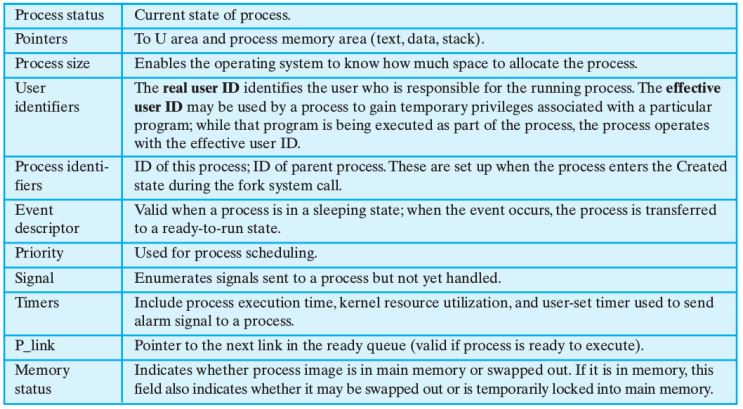
\includegraphics[width=0.50\linewidth]{images/process-table-entry.JPG}
    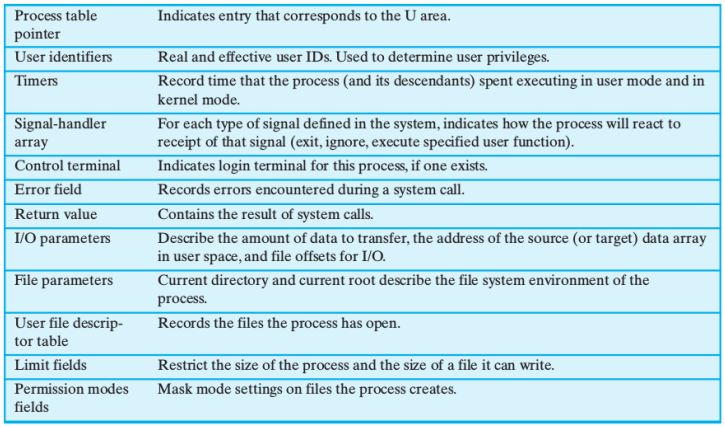
\includegraphics[width=0.49\linewidth]{images/u-area.JPG}
    \caption{Process table entry e U area}
    \label{fig:processtable-uarea}
\end{figure}

La creazione di un processo UNIX viene effettuata tramite la chiamata di sistema \verb|fork()|. In seguito a ciò, il sistema operativo, in Kernel Mode: alloca una entry nella tabella dei processi per il nuovo processo (figlio); assegna un PID unico al processo figlio; copia l'immagine del padre, escludendo dalla copia la memoria condivisa (se presente); incrementa i contatori di ogni file aperto dal padre, per tenere conto del fatto che ora sono anche del figlio; assegna al processo figlio lo stato Ready to Run; fa ritornare alla fork il PID del figlio al padre, e 0 al figlio. Dopodiché, il Kernel può scegliere tra: continuare ad eseguire il padre, switchare al figlio o switchare ad un altro processo.